\documentclass[10pt]{article}
\usepackage{graphicx}
\usepackage{amssymb}
\usepackage[fleqn]{amsmath}
\usepackage{nccmath}
\usepackage{cases}
\usepackage{hyperref}
\usepackage{multicol}
\usepackage{tikz}
\usepackage{pgfplots}
\usepackage{enumitem}
\pgfplotsset{compat=1.18}
\usepackage{float}
\usepackage{pdfpages}
\DeclareMathOperator*{\lcm}{lcm}

\title{\bf Math 116: Problem Set 4}
\date{2/5/2024}
\author{\bf Owen Jones}
\begin{document}
\maketitle
\begin{enumerate}[label= \arabic*.]
    \item $x=2+7k_1=3+10k_2\Rightarrow 7k_1-10k_2=1$. 
    By inspection, $k_1=3+10t,k_2=2+7t$. 
    Thus, $x\equiv 23\pmod{70}$.
    \item $x\equiv 1\pmod{3},x\equiv 2\pmod{4},x\equiv 3\pmod{5}$.
    $x\equiv 28\pmod{60}$ by brute force, but solvable by system of equations. 
    Smallest group is $28$. Second smallest group is $88$.
    \item $123\equiv 23\pmod{100}$. 
    $\phi(100)=100-50-20+10=40$. $23^{40}\equiv 1\pmod{100}$. 
    $123^{562}\equiv 23^2\pmod{100}\Rightarrow 123^{562}\equiv 29\pmod{100}$.
    \item \begin{enumerate}
        \item $7\equiv 3\pmod{4}$. $\phi(4)=2$. Thus, $7^7\equiv 3\pmod{4}$.
        \item $\phi(10)=10(\frac{1}{2})(\frac{4}{5})=4$. 
        Thus, $7^{7^7}\equiv 7^3\pmod{10}$ by part (a).
        $7^3=343\Rightarrow 7^{7^7}\equiv 3\pmod{10}$.
    \end{enumerate}
    \item \begin{enumerate}
        \item $\phi(1)=1,\phi(2)=1,\phi(5)=4,\phi(10)=4\Rightarrow\displaystyle\sum_{\underset{d\mid n}{1\le d\le n}} \phi(d)=10$.
        \item $\phi(1)=1,\phi(2)=1,\phi(3)=2,\phi(4)=2,\phi(6)=2,\phi(12)=4\Rightarrow\displaystyle\sum_{\underset{d\mid n}{1\le d\le n}} \phi(d)=12$.
        \item $\displaystyle\sum_{\underset{d\mid n}{1\le d\le n}} \phi(d)=n$
    \end{enumerate}
    \item \begin{enumerate}
        \item If $a$ and $n$ are coprime, then $a^{\phi(n)}\equiv 1\pmod{n}$ by Euler's Theorem. 
        Since such an integer $\phi(n)$ exists, $k\le \phi(n)$ because any $k$ larger cannot be the smallest $k$ s.t $a^k\equiv1\pmod{n}$.
        \item If $t$ is a multiple of $k$, there exists some $q$ s.t $t=kq$. 
        It follows if $a^k\equiv 1\pmod{n}\Rightarrow {(a^k)}^q=a^t\equiv 1^q\pmod{n}\Rightarrow a^t\equiv 1\pmod{n}$.
        \item If $a^t\equiv 1\pmod{n}$ then $a^{qk+r}\equiv 1\pmod{n}$. 
        Thus, $a^r\cdot a^{qk}\equiv 1\pmod{n}$. 
        However, $a^{qk}\equiv 1\pmod{n}$ by part $b$. 
        Thus, $a^r\equiv 1\pmod{n}$. 
        Since $k$ is the smallest possible positive integer s.t $a^k\equiv 1\pmod{n}$ and $0\le r<k$, $r$ must be equal to $0$ because $a^0=1$ for all $a$ coprime to $n$.
    \end{enumerate}
    \item First we show $a_i y_i z_i\equiv a_i\pmod{m_i}$. Because $y_i\equiv z_i^{-1}\pmod{m_i}\Rightarrow$ there exists some $k_i$ s.t $y_i=z_i^{-1}+m_ik_i$. 
    Thus, $a_i y_i z_i=a_i z_i^{-1}z_i+a_i z_i m_i=a_i+a_i z_i m_i\Rightarrow a_i y_i z_i\equiv a_i\pmod{m_i}$.\\
    Next we show, $a_i y_i z_i\equiv 0\pmod{m_j}$. $m_j\mid z_i m_i$ because $m_j\mid M$ and $M=z_i m_i$.
    By HW3 Q6b, $\gcd(m_i,m_j)=1$ and $m_j\mid z_i m_i\Rightarrow m_j\mid z_i$.
    Thus, $a_i y_i z_i\equiv 0\pmod{m_j}$.
    Because $x=\sum_{i=1}^{n}a_iy_iz_i$ and addition is well defined in modulo arithmetic, $\sum_{i=1}^{n}a_iy_iz_i\equiv a_i+(n-1)\cdot 0\pmod{m_i}$. 
    Hence, $x\equiv a_i\pmod{m_i}$.
    \item \begin{enumerate}
        \item $x^2\equiv 3\pmod{13},x^2\equiv 1\pmod{11}\\
        \Rightarrow x\equiv \pm4\pmod{13},x\equiv\pm 1\pmod{11}$\\
        $x=\pm(4\cdot 66+65)\equiv 43,100\pmod{143}$\\
        $x=\pm(4\cdot 66-65)\equiv 87,56\pmod{143}$\\
        $\Rightarrow x=43,100,87,56$
        \item $x^2\equiv 0\pmod{11},x^2\equiv 12\pmod{13}\\
        \Rightarrow x\equiv 0\pmod{11},x\equiv\pm 5\pmod{13}$\\
        $x=\pm 5\cdot 66\equiv 44,99\pmod{143}\\
        \Rightarrow x=44,99$
    \end{enumerate}
    \item Assume to the contrary there exists some $x$ s.t $x^2\equiv -1\pmod{p}$.
    Because $p\equiv 3\pmod{4}\Rightarrow \frac{p-1}{2}\equiv 1\pmod{4}$ i.e $\frac{p-1}{2}$ is an odd integer.
    ${(x^2)}^\frac{p-1}{2}\equiv {(-1)}^\frac{p-1}{2}\pmod{p}\Rightarrow x^{p-1}\equiv -1\pmod{p}$.
    However, $x^{p-1}\equiv 1\pmod{p}$ by Fermat's Little Theorem, so we obtain a contradiction.
    Hence, $x^2\not\equiv -1\pmod{p}$.
    \item Assume for the sake of contradiction that $m$ is a common multiple of $a$ and $b$, but $\lcm(a,b)\nmid m$.
    Division with remainder leaves quotient $q$ with remainder $r$ for integers $q$ and $\lcm(a,b)>r$.
    Because both $a$ and $b$ divide $m$ and $\lcm(a,b)$ then $a$ and $b$ divide a linear combination of $m$ and $\lcm(a,b)$. 
    Thus, $a\mid r$ and $b\mid r$.
    However, $r<\lcm(a,b)$, but by the definition of least common modulo, $a$ and $b$ can't both divide anything less than $\lcm(a,b)$.
    Hence, we obtain a contradiction, so $\lcm(a,b)\mid m$.
    \item \begin{enumerate}
        \item Let $p$ be prime, and suppose for the sake of contradiction $p\mid n$ and $p\mid k$. 
        It follows $n=pq_1$ and $k=pq_2$ for integers $q_1$ and $q_2$.
        Thus, $pg\mid a$ and $pg\mid b$. 
        However, $g$ is the greatest common divisor of $a$ and $b$, but $g<pg$ because $p>1$.
        Thus, we obtain a contradiction, so $n$ and $k$ must be coprime.
        \item $ngk$ is a multiple of $a$ because there exists an integer $k$ s.t $ak=ngk$. 
        Similarly, $ngk$ is a multiple of $b$ because there exists an integer $n$ s.t $an=ngk$.
        Because $ngk$ is a multiple of $a$ and $b$, $ngk$ is a common multiple of $a$ and $b$.
        \item If $m$ is a common multiple of $a$ and $b$, then $a\mid m$ and $b\mid m$. 
        Let $m=gq$ for some integer $q$. 
        We claim $n\mid q$ and $k\mid q$.
        Because $a\mid m$ there exists some integer $q_1$ s.t $q_1ng=gq$.
        Cancelling $g$ on both sides, we obtain $q_1n=q$. 
        Since $q$ is a multiple of $n$, then $n\mid q$.
        We use the same approach to show $k\mid q$.
        Since $n$ and $k$ are coprime, $\lcm(n,k)=nk$.
        By 10, $nk\mid q\Rightarrow gnk\mid m$.
    \end{enumerate}
    \item  %Let $g=\gcd(n_1,n_2)$. WTS that for $x$ to have a solution, then $a_1\equiv a_2\pmod{g}$. 
    % $x\equiv a_1\pmod{g}$ and $x\equiv a_2\pmod{g}$ because $\gcd(n_1,n_2)$ divides both $n_1$ and $n_2$.
    % By transitivity, $a_1\equiv a_2\pmod{g}$. Thus, for rest of the proof we have $g\mid (a_1-a_2)$.
    % From Bezout's identity, there exists integers $y_1,y_2$ s.t $n_1y_1+n_2y_2=g$.
    % Because $n_1$ and $n_2$ are both divisible by $g$, we obtain $\frac{n_1}{g}y_1+\frac{n_2}{g}y_2=1$.
    % Next, we want to show $x=a_1\frac{n_2}{g}y_2+a_2\frac{n_1}{g}y_1$ is a valid solution.
    % From Bezout's identity $\frac{n_1}{g}y_1=1-\frac{n_2}{g}y_2$. 
    % It follows $x=a_1\frac{n_2}{g}y_2+a_2-a_2\frac{n_2}{g}y_2\equiv a_2\pmod{n_2}$ because $n_2\mid\frac{a_1-a_2}{g}n_2y_2$.
    % Similarly, we can show $x\equiv a_1\pmod{n_1}$. Thus, $x$ is a valid solution.
    Suppose $x$ and $x'$ are both valid solutions. 
    By transitivity $x\equiv x'\pmod{n_1}$ and $x\equiv x'\pmod{n_2}$.
    Thus $n_1\mid (x-x')$ and $n_2\mid (x-x')$. 
    It follows $(x-x')$ is a common multiple of $n_1$ and $n_2$.
    Thus, $\lcm(n_1,n_2)\mid (x-x')$. Hence, $x\equiv x'\pmod{l}$.
    \item \begin{enumerate}
        \item Let $g=\gcd(a,b)$. Because $g\mid a$ and $g\mid b$, it follows $g\mid r$. 
        Thus, $g$ is a divisor of both $b$ and $r$.
        Suppose $d$ is some divisor of both $b$ and $r$.
        It follows $d$ divides a linear combination of $b$ and $r$.
        Thus, $d\mid a$.
        However, $d\le g$ because $g$ is the $\gcd(a,b)$.
        Hence, because $g$ also divides $b$ and $r$, $\gcd(a,b)=\gcd(b,r)$
        \item The Euclidean Algorithm terminates after $n$ steps when we obtain $r_{n-1}=q_n r_n+0$. 
        Inductively, we can show $\gcd(a,b)=\gcd(r_n,0)=r_n$.
    \end{enumerate}
    \item $x\equiv 26663845164692\pmod{41852119381815}$
    \item $x\equiv 7543804279237\pmod{24547393284917}$
\end{enumerate}
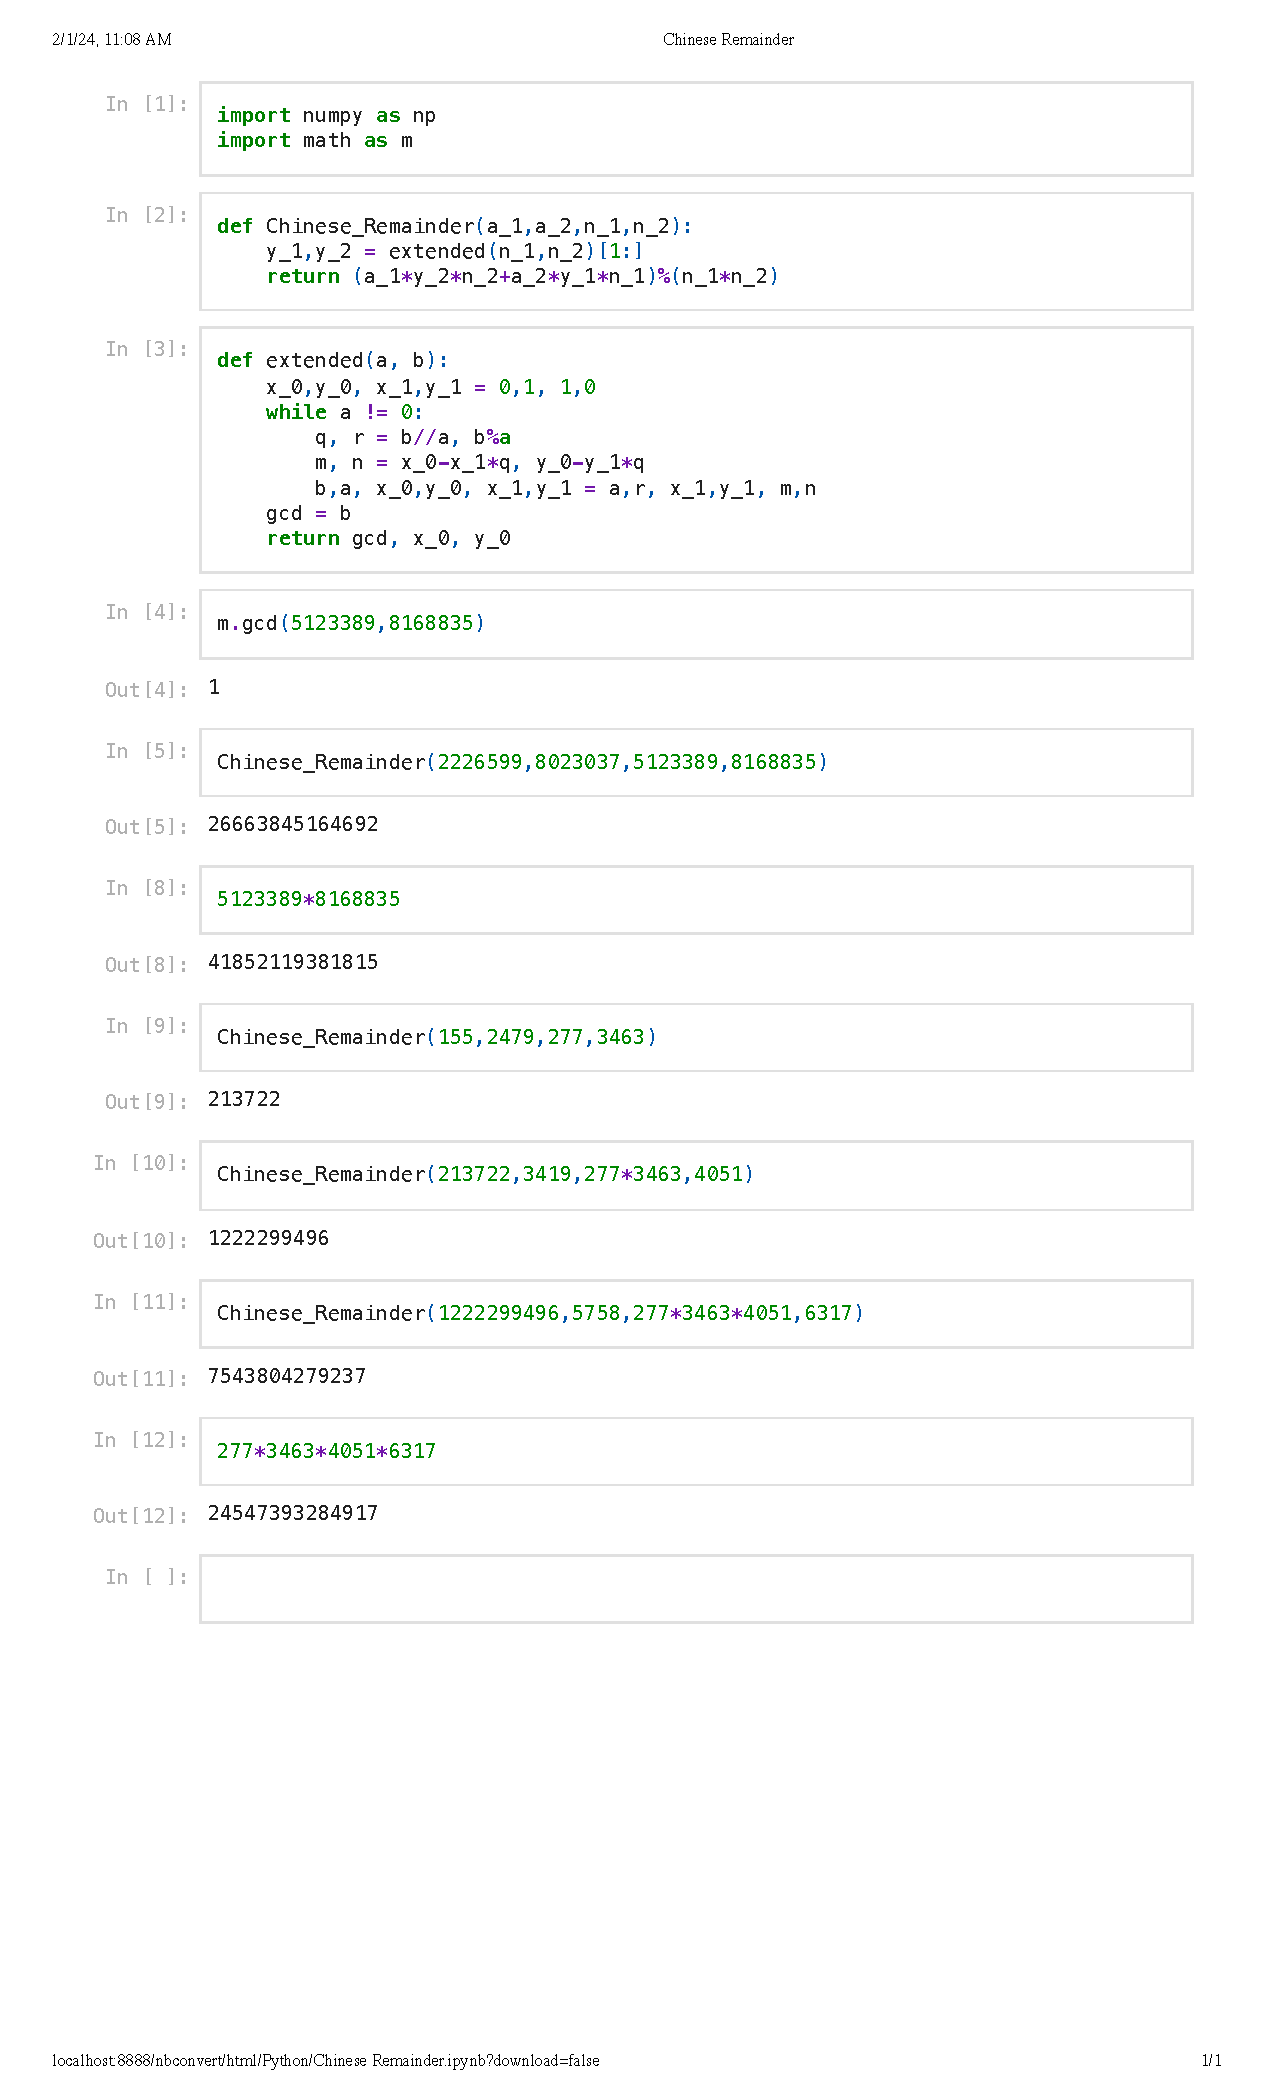
\includepdf{Chinese Remainder.pdf}
\end{document}